\documentclass{beamer}



%\usetheme{Marburg}
\usetheme{Berlin}

\usepackage{geometry}

\usepackage[english, ngerman]{babel}
\usepackage[T1]{fontenc}
\usepackage[utf8]{inputenc}

\usepackage{amsmath}                     % macht
\usepackage{amsfonts}                     %          mathe
\usepackage{amssymb}                     %                   mächtiger

\usepackage[]{units}
\usepackage{gensymb}
\usepackage{pifont}

\usepackage{appendixnumberbeamer}

\usepackage{multimedia}
\usepackage{color}
\usepackage{ifthen}
\usepackage{animate}

\usepackage{tikz}
\usetikzlibrary{positioning}
\usetikzlibrary{shadings}
\usetikzlibrary{fadings}
\usetikzlibrary{arrows}
\usetikzlibrary{decorations.markings}

\usepackage[framemethod=tikz]{mdframed}

\newcounter{angle} % ???
\setcounter{angle}{0} % ???

\setbeamercovered{transparent}
\setbeamercovered{dynamic}

\def\insertframetitle{}

%\definecolor{lkb}{RGB}{100,100,100}
\definecolor{lkb}{RGB}{0,162,212}
\definecolor{my_green}{RGB}{105, 184, 73}
\definecolor{my_red}{RGB}{244, 131, 107}


\setbeamercolor{secsubsec}{fg=lkb,bg=lkb}
\setbeamercolor{shadow}{fg=lkb,bg=lkb}

\setbeamercolor{block title}{use=structure,fg=white,bg=lkb}
\setbeamercolor{block body}{use=structure,fg=black,bg=lkb!20!white}

\setbeamercolor{block title example}{use=structure,fg=white,bg=my_green}
\setbeamercolor{block body example}{use=structure,fg=black,bg=my_green!20!white}

\setbeamercolor{block title alerted}{use=structure,fg=white,bg=my_red}
\setbeamercolor{block body alerted}{use=structure,fg=black,bg=my_red!20!white}



\setbeamertemplate{items}[circle]

\usepackage{epic}
\usepackage{graphicx}
\usepackage[percent]{overpic}
\usepackage{pict2e}

\usepackage{ragged2e}

\beamertemplatenavigationsymbolsempty

%--------------------- TO SHOW TOC AT BEGINNING OF EACH SECTION -----------------------
\AtBeginSection[]
{
   \begin{frame}
       \frametitle{Outline}
       \tableofcontents[currentsection]
   \end{frame}
}
%-----------------------------------------------------------------------------------------------------------

%--------------------- TO CUSTOMIZE THE APPEARANCE OF TOC -------------------------------
\setbeamertemplate{section in toc}{%
  {\color{black}\inserttocsectionnumber.}~{\color{lkb}\inserttocsection}}
\setbeamercolor{subsection in toc}{bg=white,fg=structure}
\setbeamertemplate{subsection in toc}{%
  \hspace{1.2em}\textcolor{lkb}{$\blacktriangleright$}~{\color{lkb}\inserttocsubsection\par}}
%-----------------------------------------------------------------------------------------------------------

%--------------------- TO DEFINE HEADER AND FOOTER -----------------------------------------
\setbeamertemplate{headline}
{
\leavevmode
  \begin{beamercolorbox}[wd=\paperwidth,ht=0.5cm,dp=0.2cm]{secsubsec}
    \raggedright
    \hspace*{0.2cm}
    {\sffamily\large\color{white}\insertsection\hfill\insertframetitle}
    \hspace*{0.2cm}
  \end{beamercolorbox}
  \tikz\draw[draw=none,top color=lkb,bottom color=lkb!20] (0,0) rectangle (\paperwidth,0.1);
}


\setbeamertemplate{frametitle}{}

\setbeamertemplate{footline}
{
  \leavevmode
     \begin{beamercolorbox}[sep=0.3cm,ht=1.8em,wd=\paperwidth]{}

%         \raisebox{-1.45mm}{\includegraphics[width=2cm]{logo_LKB.png}}
        \begin{tikzpicture}[>=stealth]
	            \draw [lkb,line width=1pt,path fading=east] (0,0) --(11,0);
 	 \end{tikzpicture}\hfill\raisebox{-0.05cm}{{\color{lkb}\insertframenumber/\inserttotalframenumber}}	
    \end{beamercolorbox}
}
%-----------------------------------------------------------------------------------------------------------

\makeatletter
\newlength\beamerleftmargin
\setlength\beamerleftmargin{\Gm@lmargin}
\makeatother

\graphicspath{{figures/}}


\usepackage{biblatex}

%-----------------------------------------------------------------------------------------------------------
%---- START OF DOCUMENT -------------------------------------------------------------------------
%-----------------------------------------------------------------------------------------------------------

\begin{document}

{
\begin{frame}[t,plain,noframenumbering]
	\vspace{0.7cm}
	\begin{mdframed}[tikzsetting={draw=lkb,fill=white,fill opacity=0.7, line width=4}, backgroundcolor=none, 							   leftmargin=0, rightmargin=0, innertopmargin=10]
		\vspace{0.5cm}
		{\Large{
  		\begin{center}Chaos Company\\[0.25cm]
                      \rule{5cm}{0.1cm}\\[0.25cm]
                      Status
        \end{center}
		}}
  		\vspace{0.75cm}
  		\centering
  		{\small{
  		\hspace{1cm} Johannes \hspace{1cm}\phantom{}\\
  		\phantom{}\hspace{1cm} 02/04/2020 \hspace{1cm}\phantom{}\\
  		}}
	\end{mdframed}

\end{frame}
}

\begin{frame}
\frametitle{Inhalt}
\tableofcontents[]
\end{frame}

%%%%%%%%%%%%%%%%%%%%%%%%%%%%%%%%%%%%%%%
\section{Spasspatent}
%%%%%%%%%%%%%%%%%%%%%%%%%%%%%%%%%%%%%%%

%-----------------------------------------------------------------------------------------------------------
\begin{frame}{W\"urfel auf Touchscreen}



\begin{block}{Motivation:}
Test des Patentprozesses: Versuche ein (nicht besonders gutes) Patent anzumelden um Erfahrung zu sammeln
\end{block}


\begin{exampleblock}{Idee 1:}
Preparierter W\"urfel welcher durch Touchscreen erkannt wird
\end{exampleblock}

\begin{alertblock}{Potential:}
Kann in jedem Brettspiel/W\"urfelspiel genutzt werden um die Haptik des W\"urfelns beizubehalten, und trotzdem mit Leuten zu spielen welche nicht im selben Raum sitzen.\\
Geringer technischer Aufwand, idealerweise auf bereits vorhanden Ger\"aten nutzbar, aber W\"urfel werden \"uber uns bezogen.
\end{alertblock}

\end{frame}
%-----------------------------------------------------------------------------------------------------------


%%%%%%%%%%%%%%%%%%%%%%%%%%%%%%%%%%%%%%%
\section{Pandemieprognose}
%%%%%%%%%%%%%%%%%%%%%%%%%%%%%%%%%%%%%%%

%-----------------------------------------------------------------------------------------------------------
\begin{frame}{Welche Gr\"ossen?}

\begin{exampleblock}{Idee 1:}
Geburtenrate steigt in 9Monaten, Erstgeborene, keine supercleveren Eltern
\end{exampleblock}

\begin{exampleblock}{Idee 2:}
Soziale Medien nach Neuentwicklungen durchk\"ammen\\
$\rightarrow$ Philipp? Erlaubnis zu nutzen seitens Uni?
\end{exampleblock}

\begin{exampleblock}{Idee 3:}
Verschiedene L\"ander, verschiedene G\"uter werden nachgefragt
\end{exampleblock}

\begin{alertblock}{Zweite Welle?}
Kommt eine zweite Welle? Selbst wenn nicht: Arbeits- und Sozialverhalten wird sich dauerhaft \"andern? Je l\"anger der momentane Zustand andauert, umso wahrscheinlicher.
\end{alertblock}

\end{frame}
%-----------------------------------------------------------------------------------------------------------


%-----------------------------------------------------------------------------------------------------------
\begin{frame}{Schaue nach China}

\begin{center}
    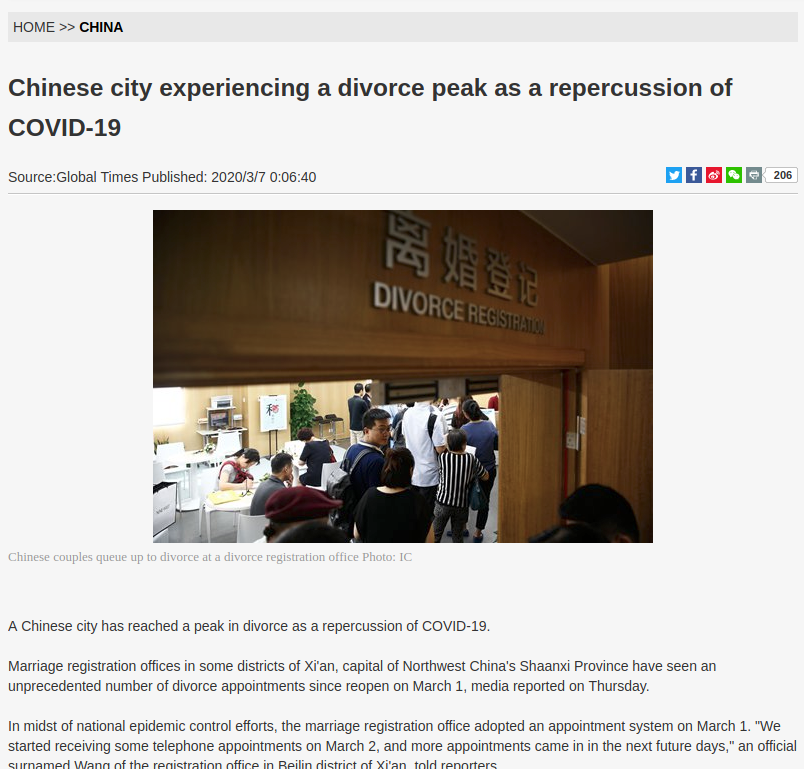
\includegraphics[width=0.45\textwidth]{fig_divorce_china}
    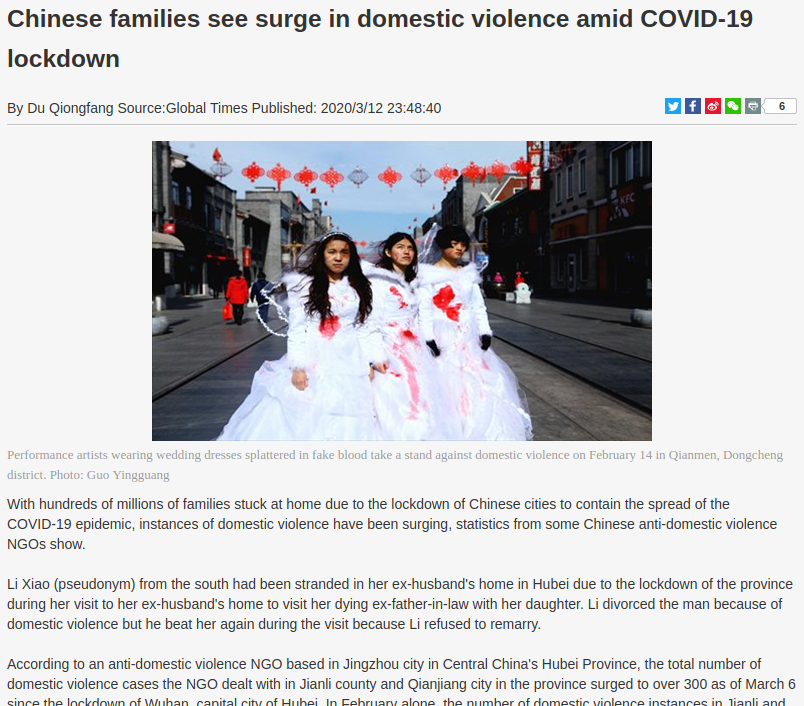
\includegraphics[width=0.45\textwidth]{fig_dom_violence_china}
\end{center}

\begin{alertblock}{China ist nicht Deutschland!}
\begin{itemize}
 \item Welches Land/welche Gr\"ossen guter Indikator?
 \item Woher Daten statt Zeitungsartikel?
\end{itemize}
\end{alertblock}

\end{frame}
%-----------------------------------------------------------------------------------------------------------


%%%%%%%%%%%%%%%%%%%%%%%%%%%%%%%%%%%%%%%
\section{Der Kniffelbot}
%%%%%%%%%%%%%%%%%%%%%%%%%%%%%%%%%%%%%%%

%-----------------------------------------------------------------------------------------------------------
\begin{frame}{Was?}

\begin{block}{Was ist Kniffel?}
Kniffel (oder Yahtzee) ist ein W\"urfelspiel mit f\"unf W\"urfeln, einem W\"urfelbecher und einem speziellen Spielblock.
\end{block}

\begin{columns}[]
  \begin{column}{0.55\textwidth}
 
    \begin{exampleblock}{Idee}
    \justifying
    Das Eintragen und Zusammenz\"ahlen der gew\"urfelten Zahlen ist zeitraubend. Mittels einer Kamera und passender Software kann das automatisiert werden.\\
    Mittels eines Kniffelbots kann auch mit Menschen am anderen Ende der Welt gespielt werden.
    \end{exampleblock}
	
  \end{column}
  \begin{column}{0.35\textwidth}
  
    \begin{center}
        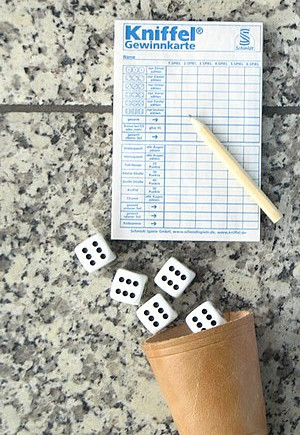
\includegraphics[width=0.8\textwidth]{fig_kniffel}
    \end{center}
	
  \end{column}
\end{columns}


\end{frame}
%-----------------------------------------------------------------------------------------------------------

%-----------------------------------------------------------------------------------------------------------
\begin{frame}{Status}

\begin{center}
    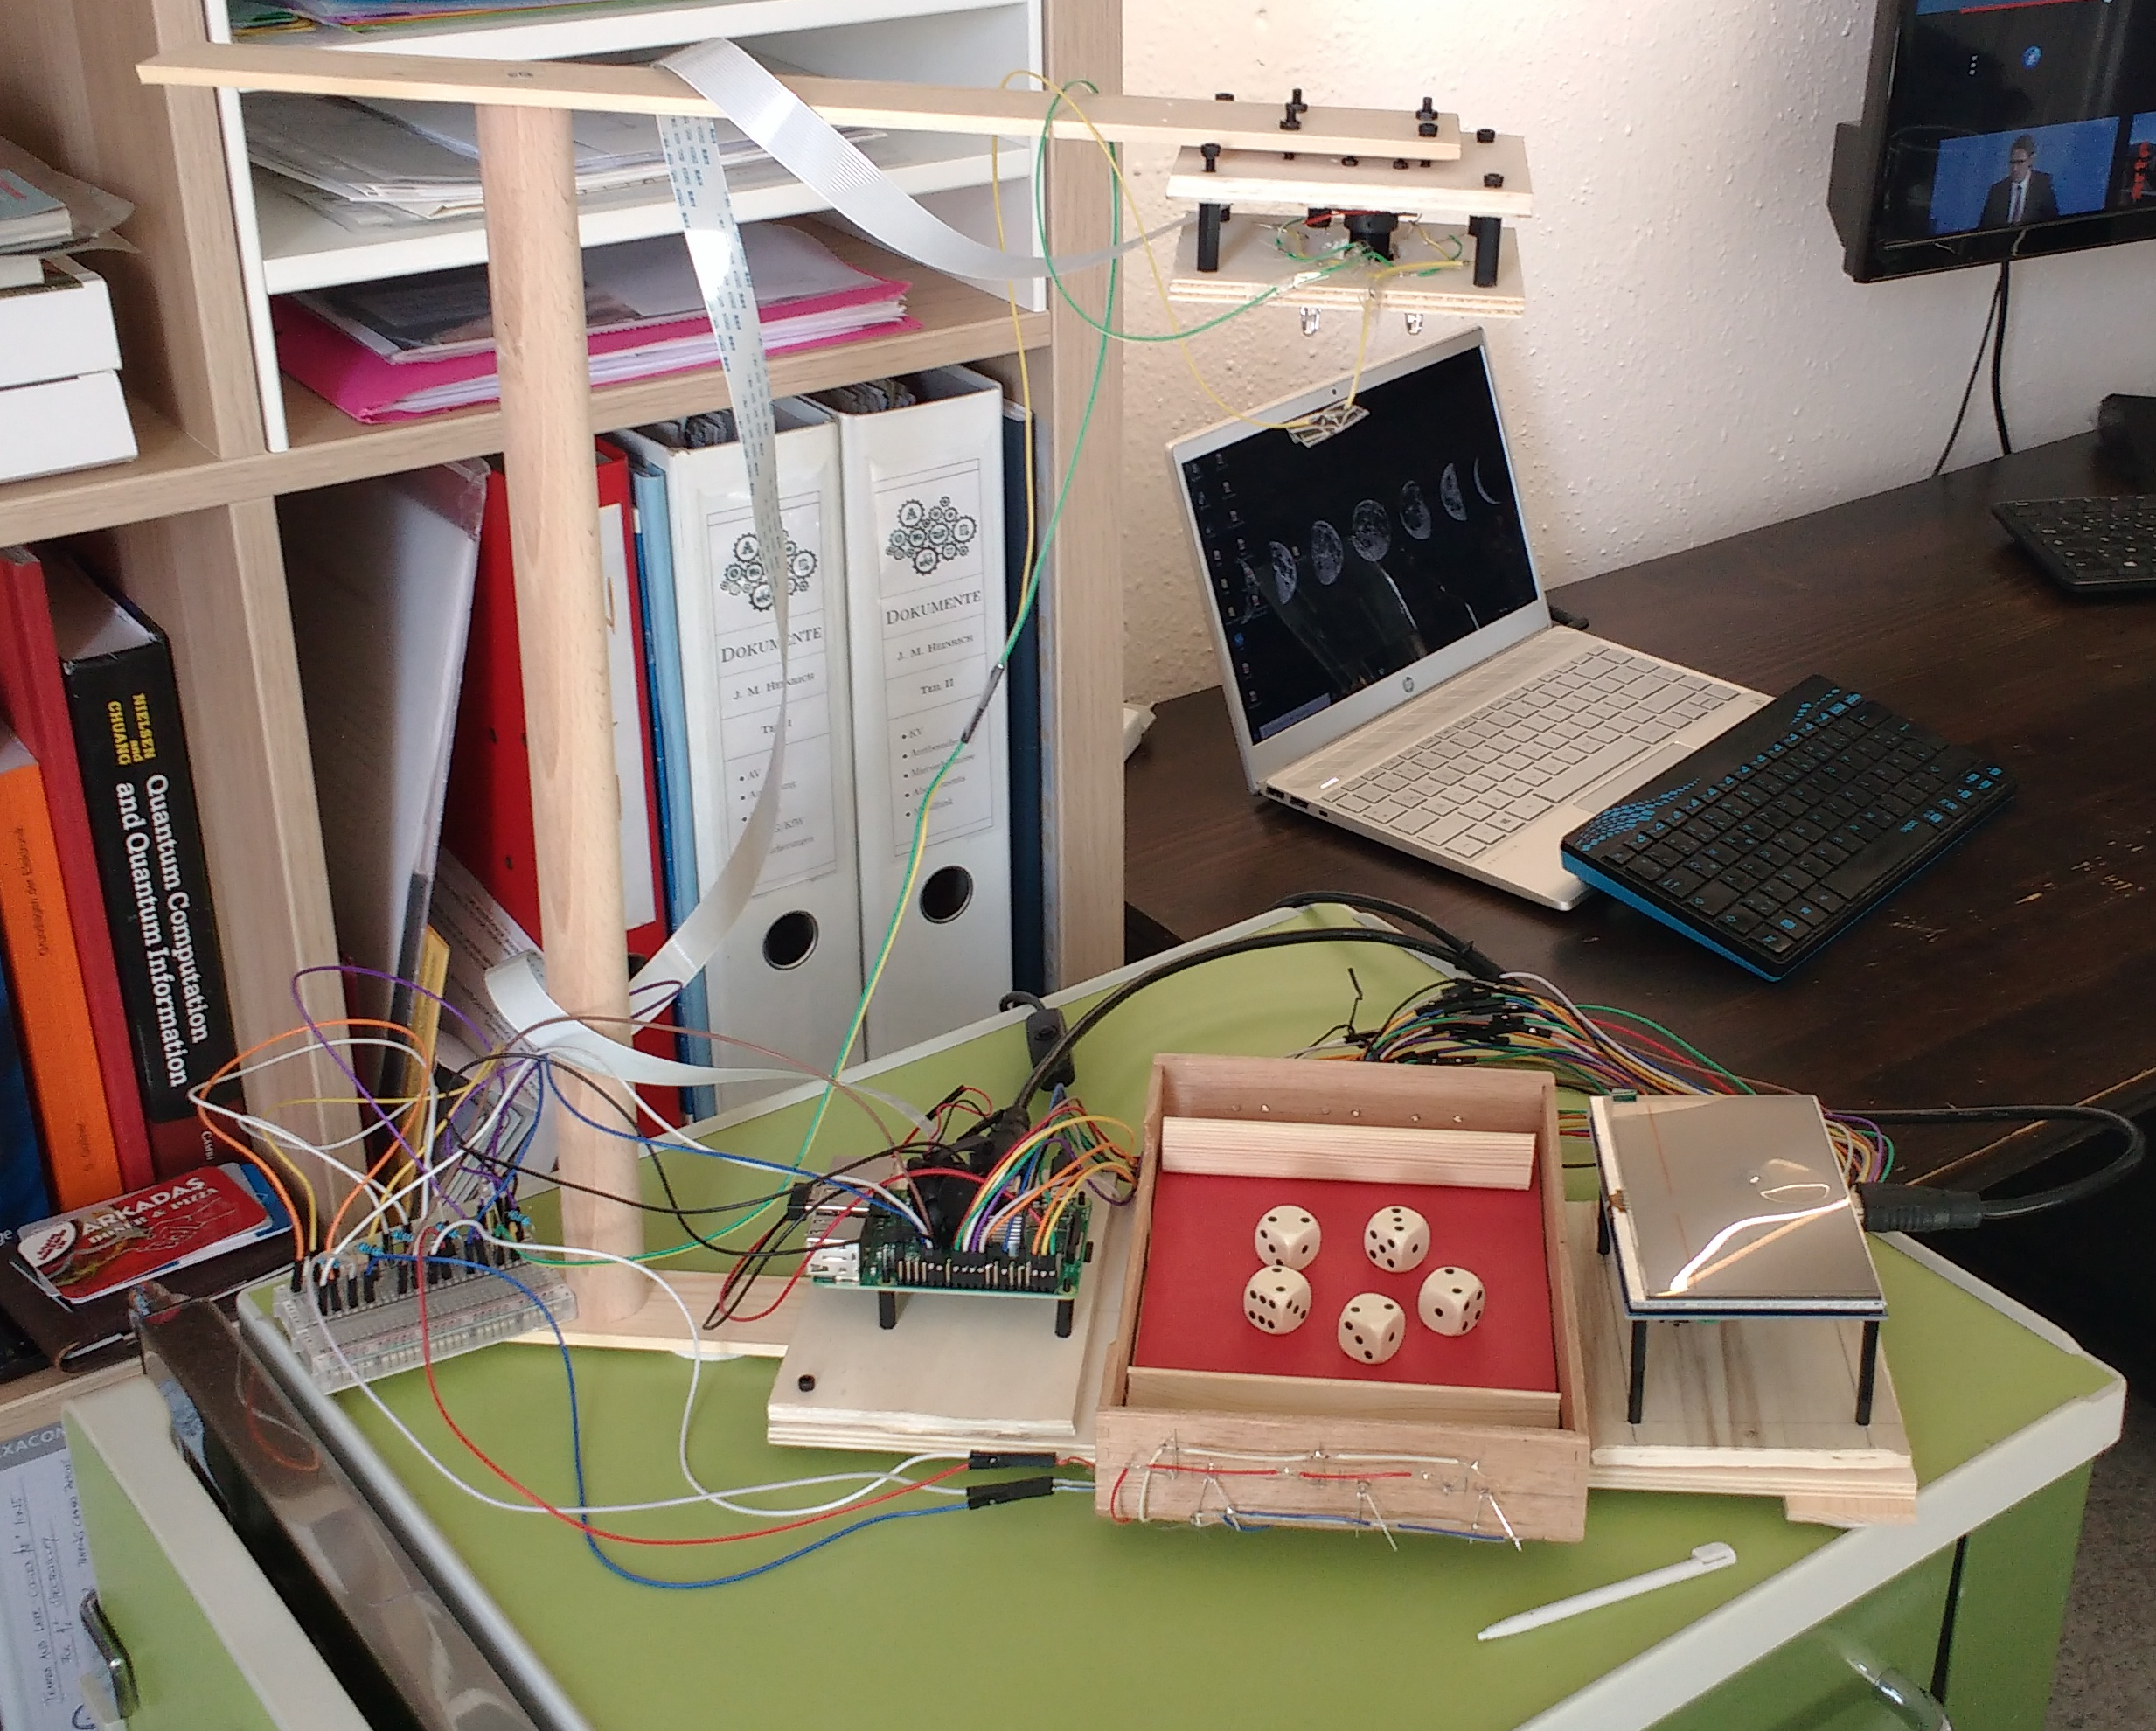
\includegraphics[width=0.45\textwidth]{fig_kniffelbot_1}
    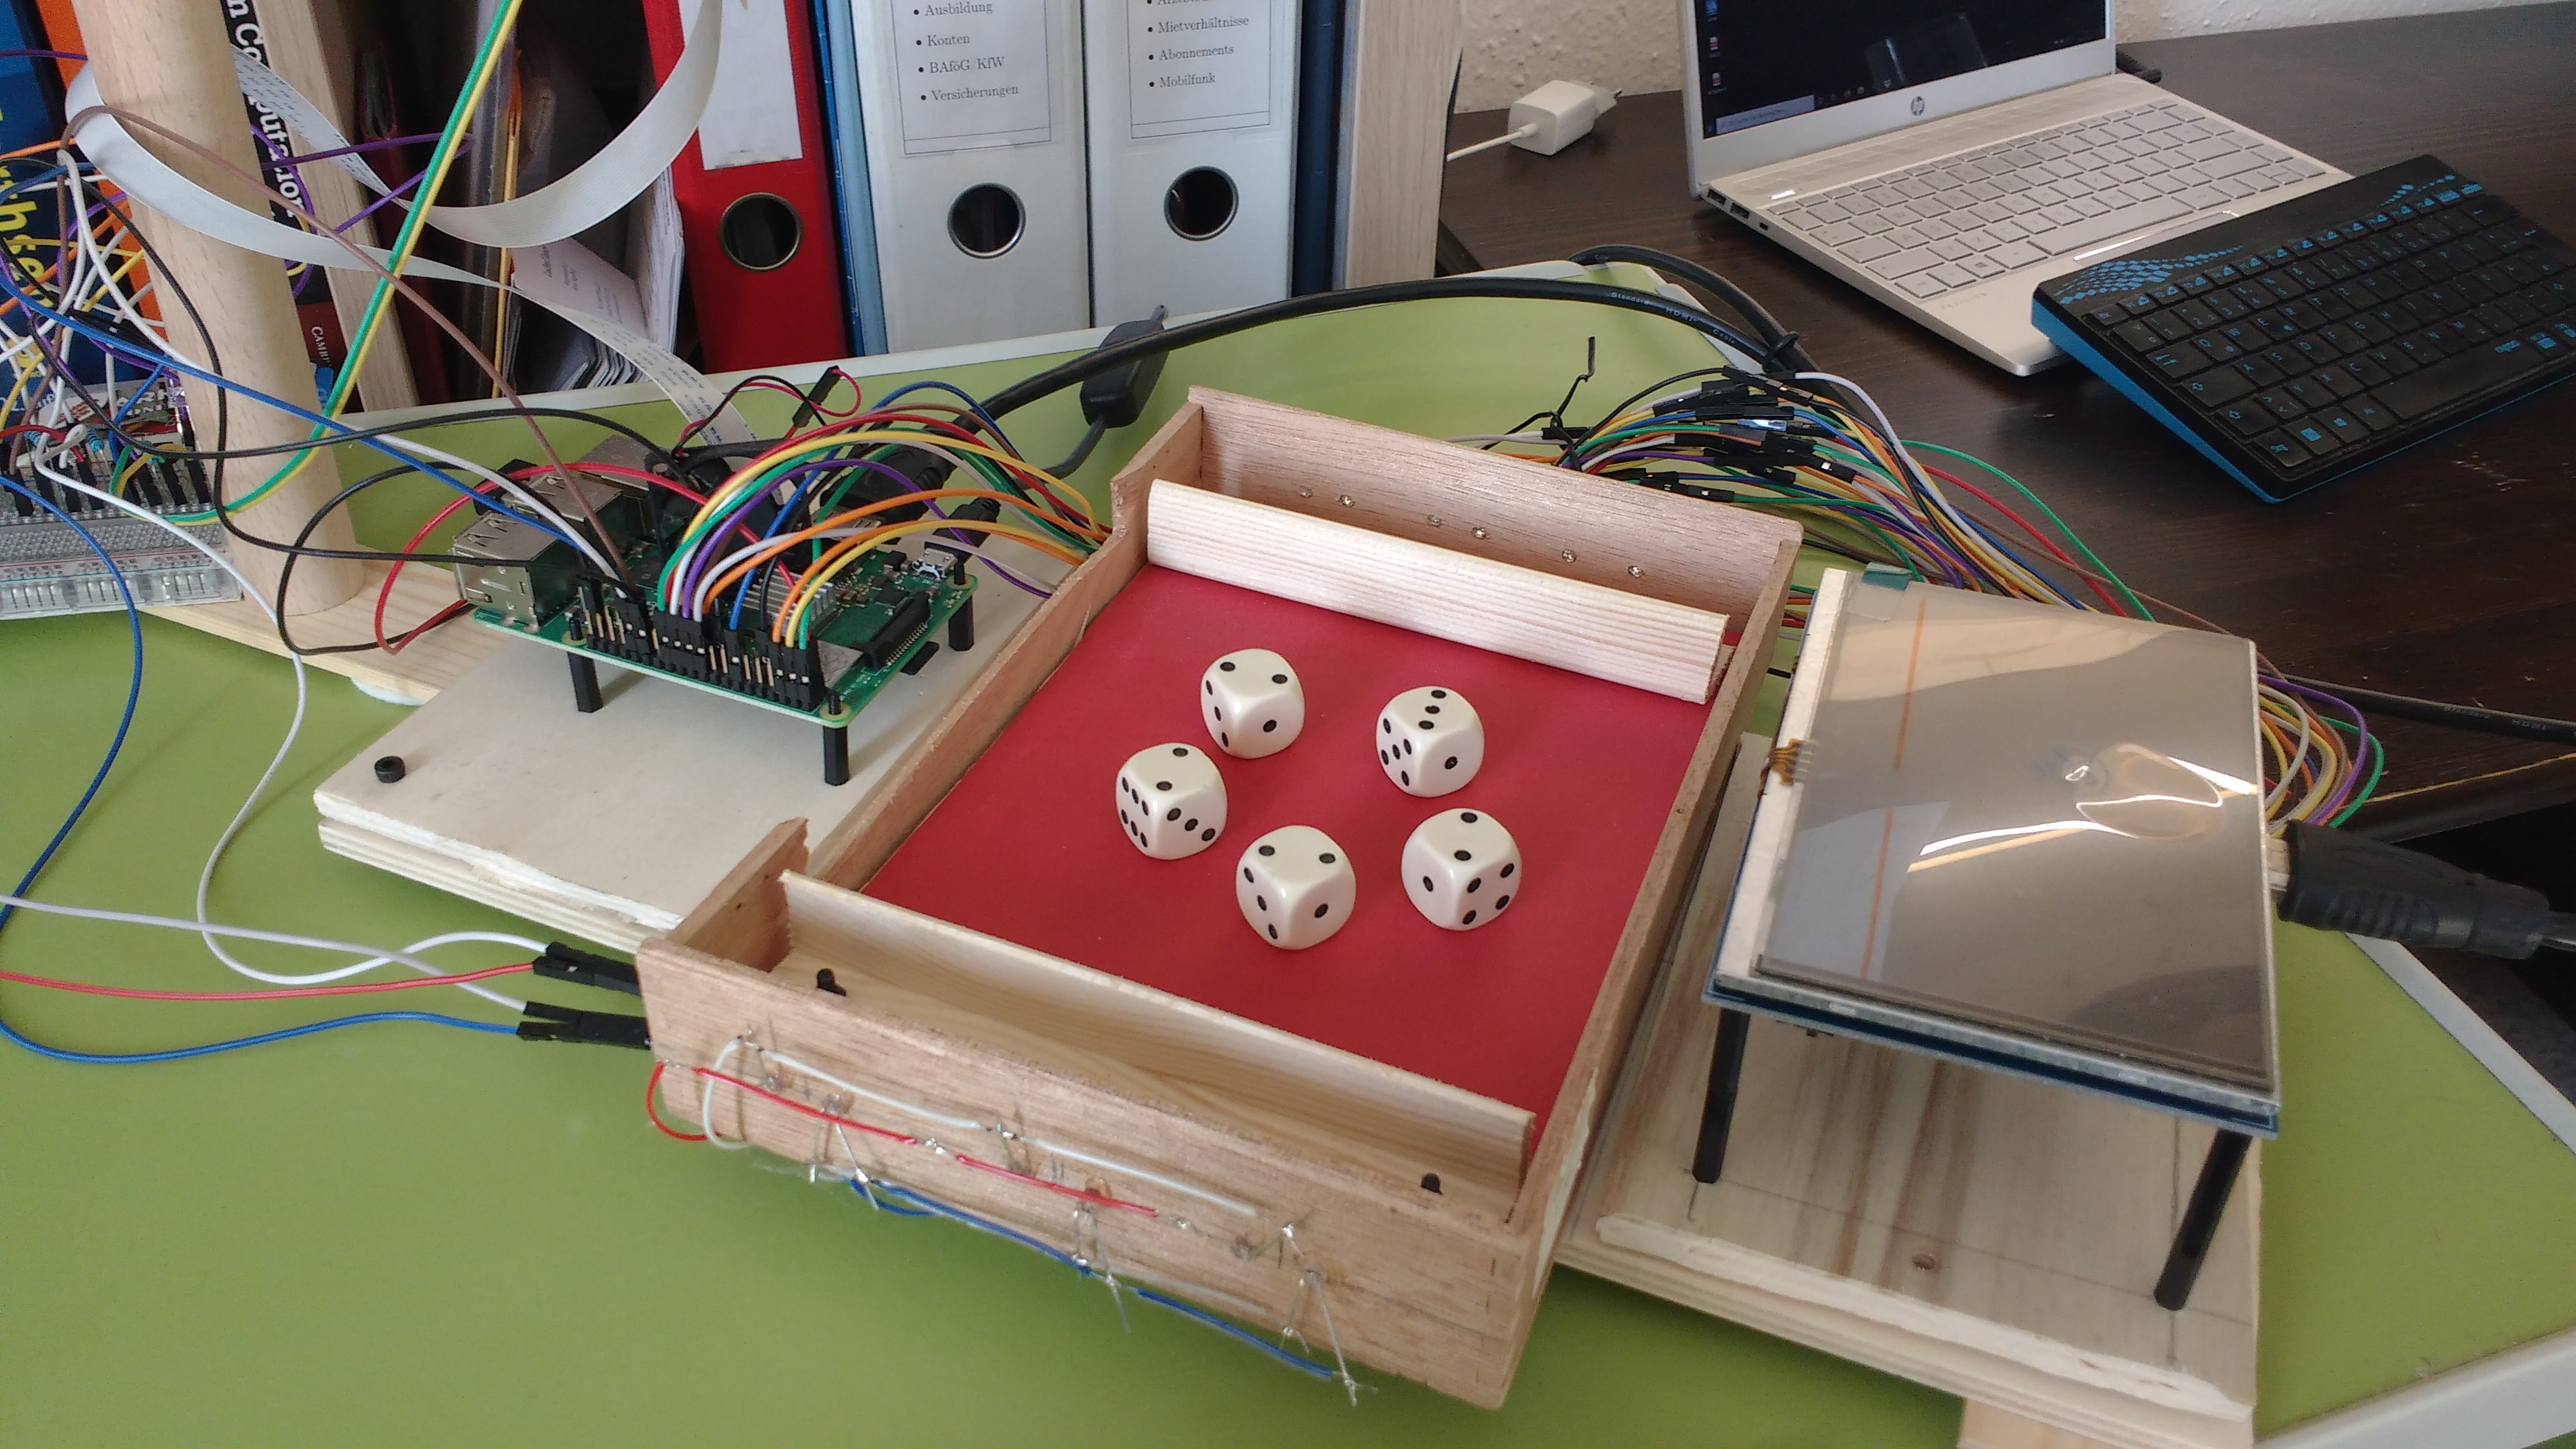
\includegraphics[width=0.45\textwidth]{fig_kniffelbot_2}
\end{center}

\end{frame}
%-----------------------------------------------------------------------------------------------------------

%-----------------------------------------------------------------------------------------------------------
\begin{frame}{Status}

\begin{center}
    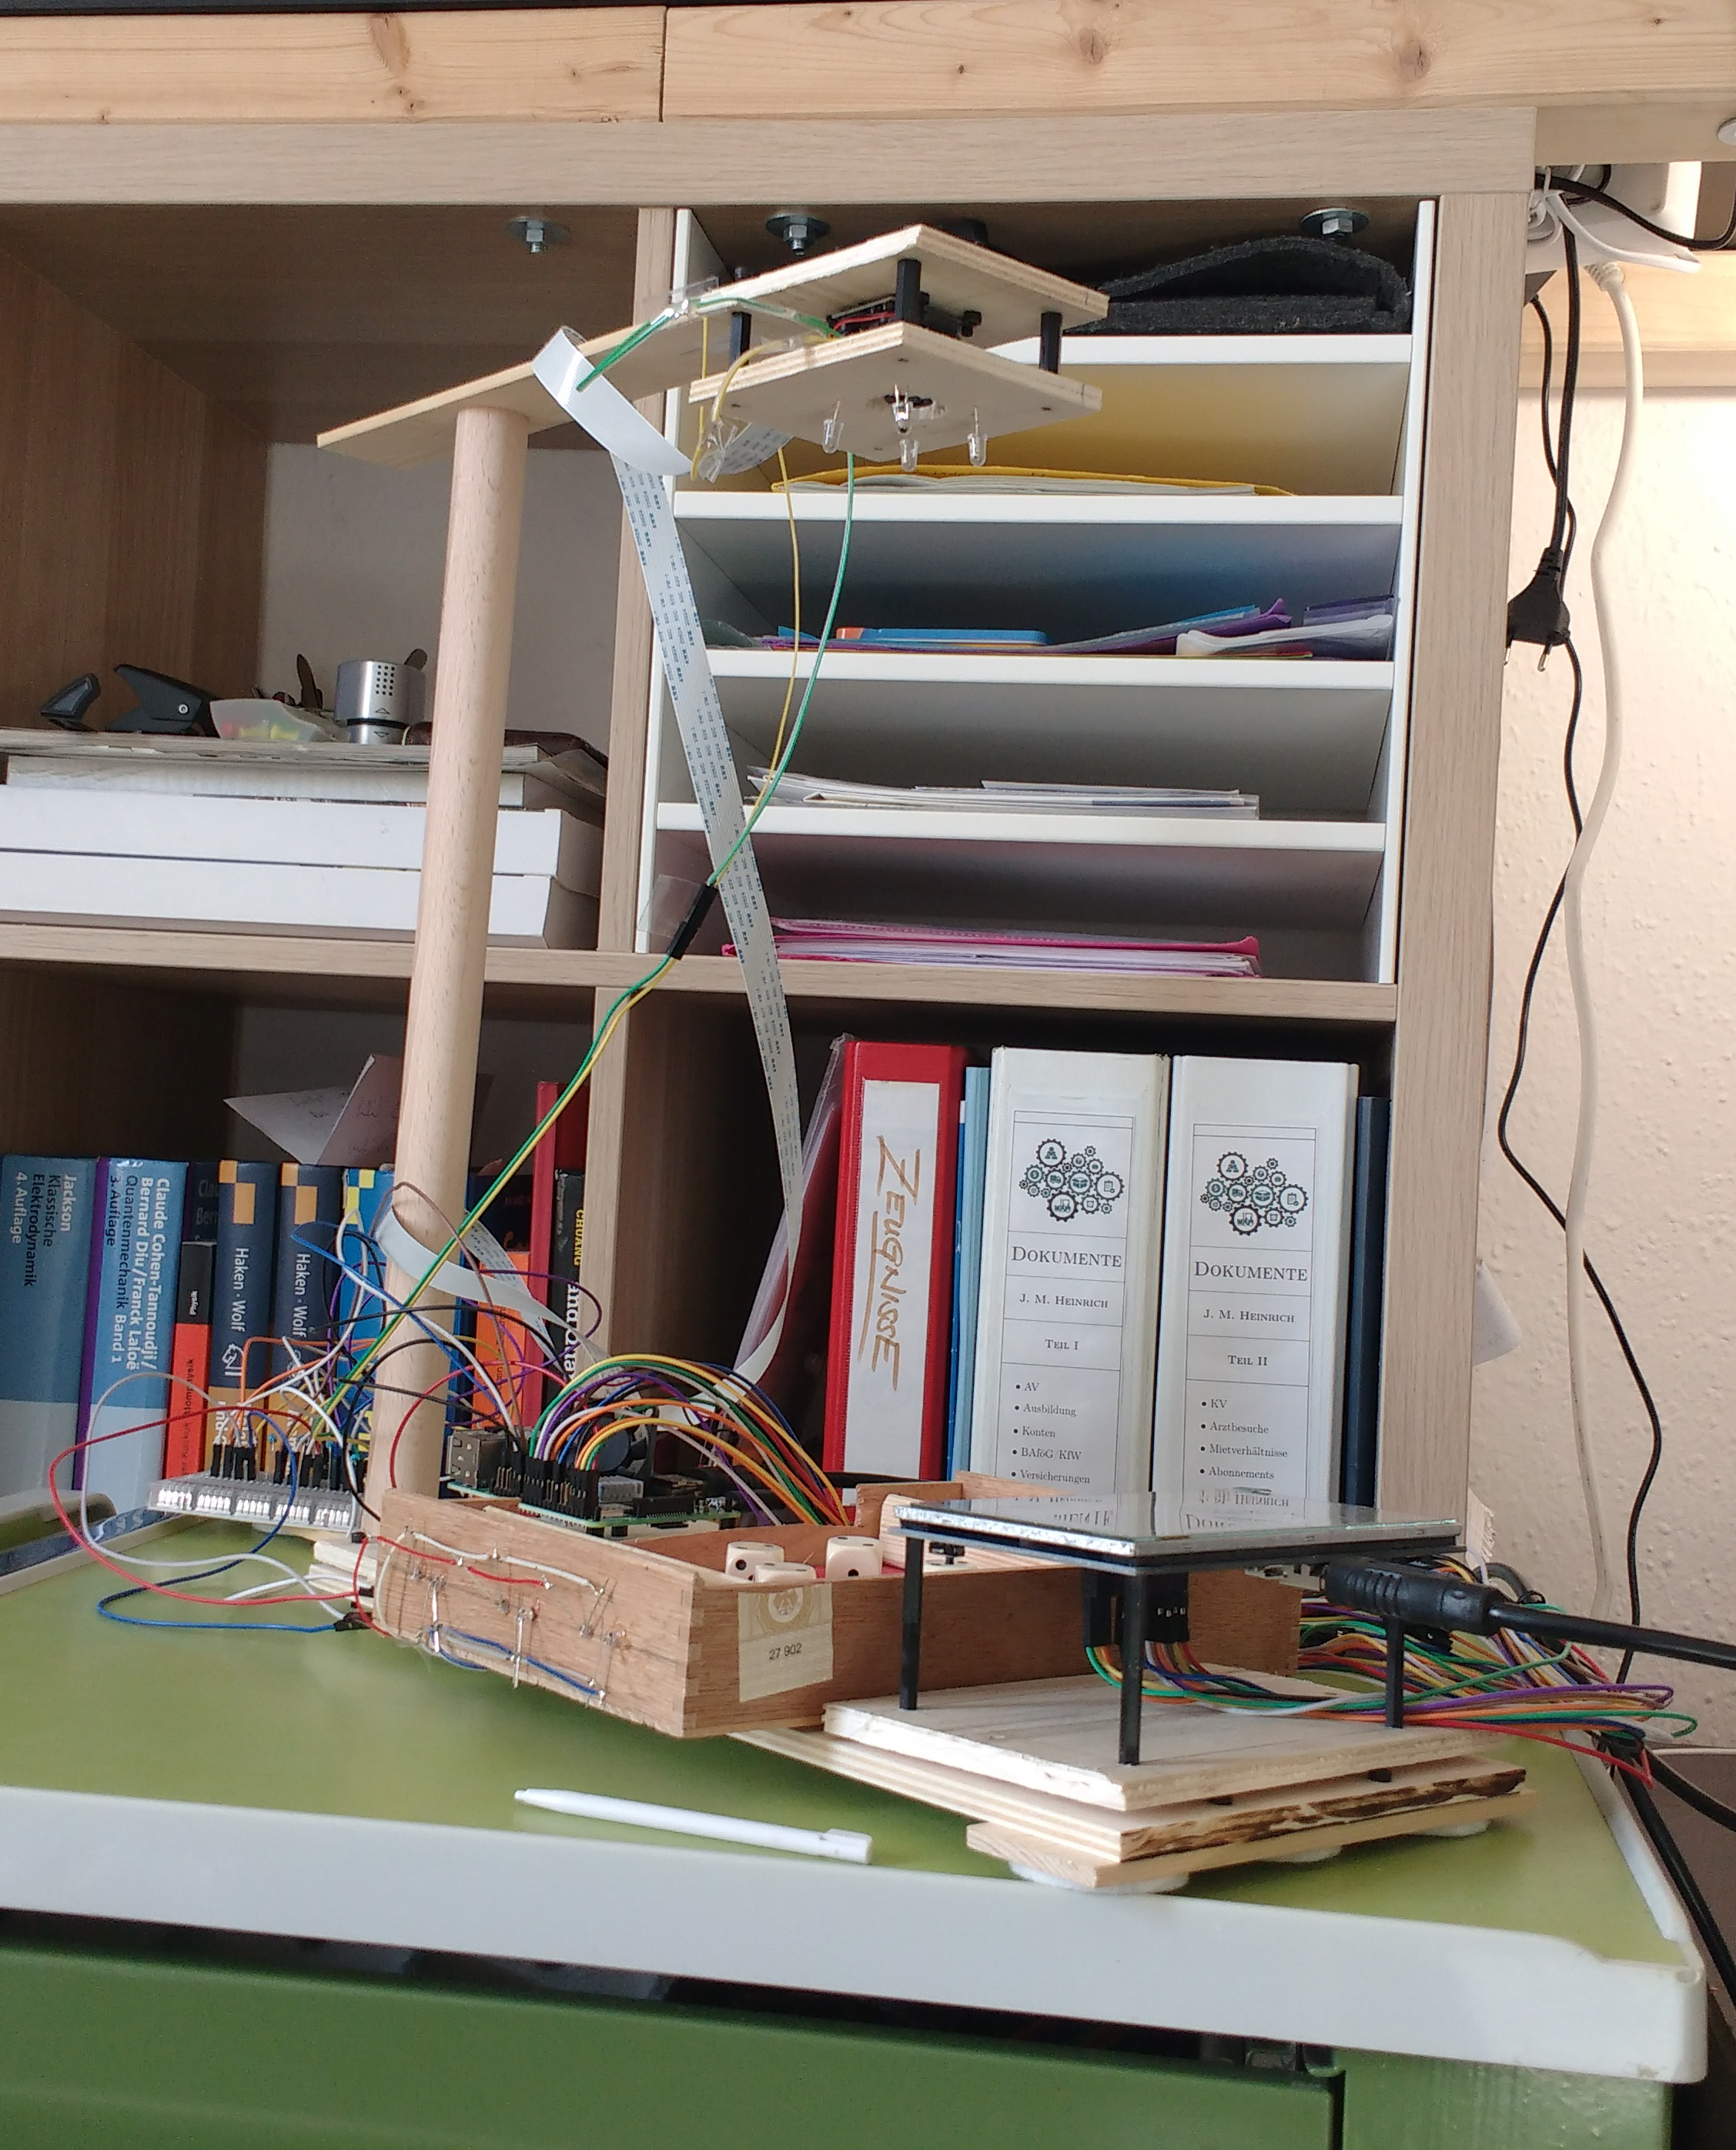
\includegraphics[width=0.45\textwidth]{fig_kniffelbot_3}
    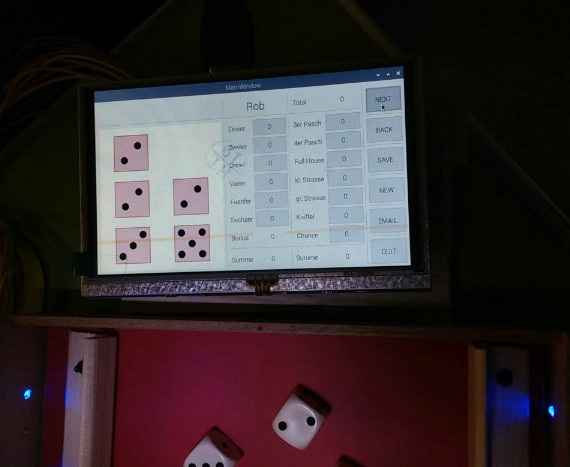
\includegraphics[width=0.45\textwidth]{fig_kniffelbot_4}
\end{center}

\end{frame}
%-----------------------------------------------------------------------------------------------------------


%-----------------------------------------------------------------------------------------------------------
\begin{frame}{Status}

\begin{center}
    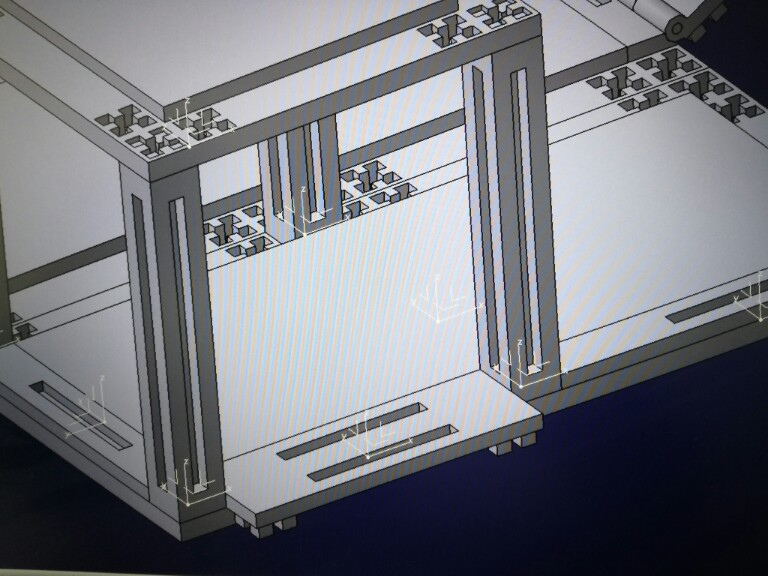
\includegraphics[width=0.45\textwidth]{fig_kniffelbot_5}
    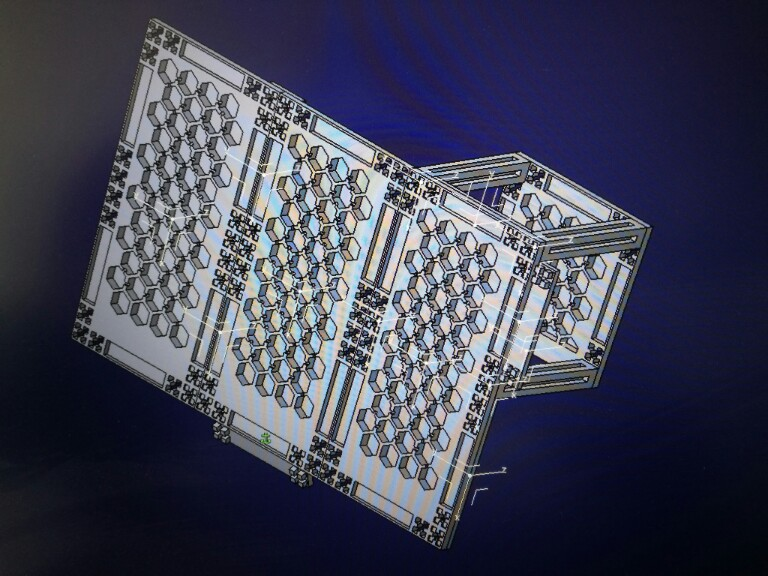
\includegraphics[width=0.45\textwidth]{fig_kniffelbot_6}
    
    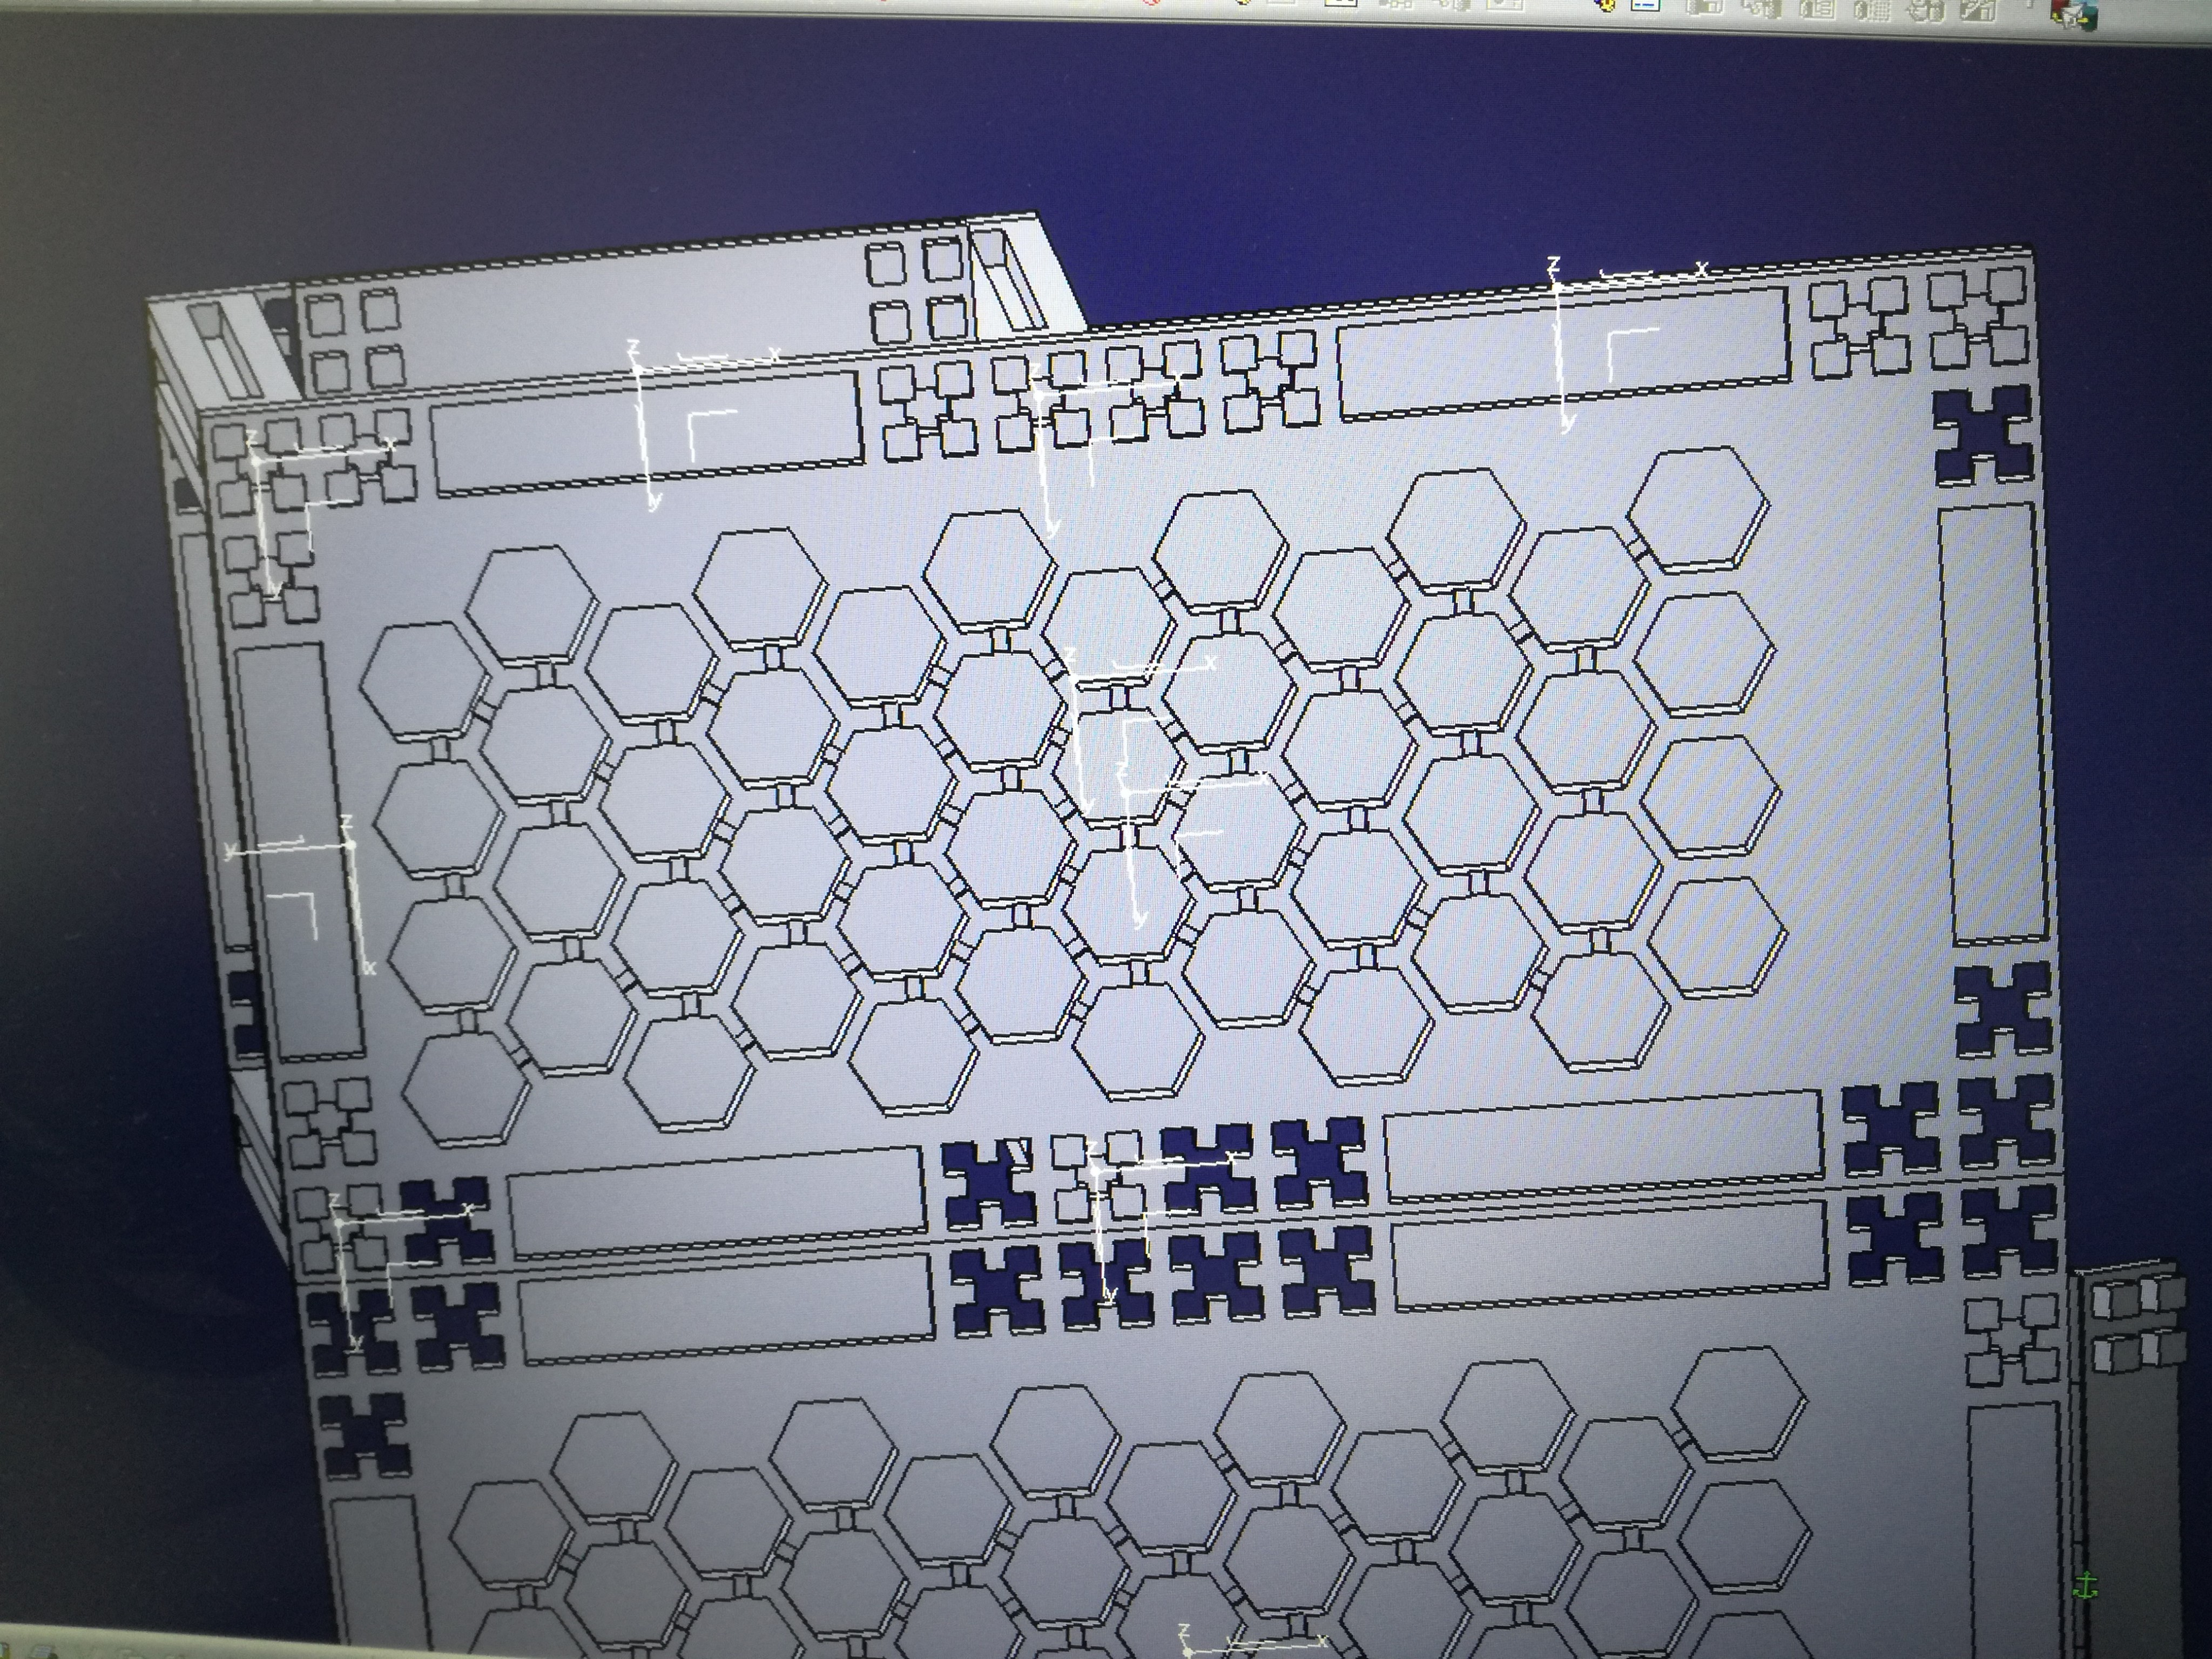
\includegraphics[width=0.45\textwidth]{fig_kniffelbot_7}
    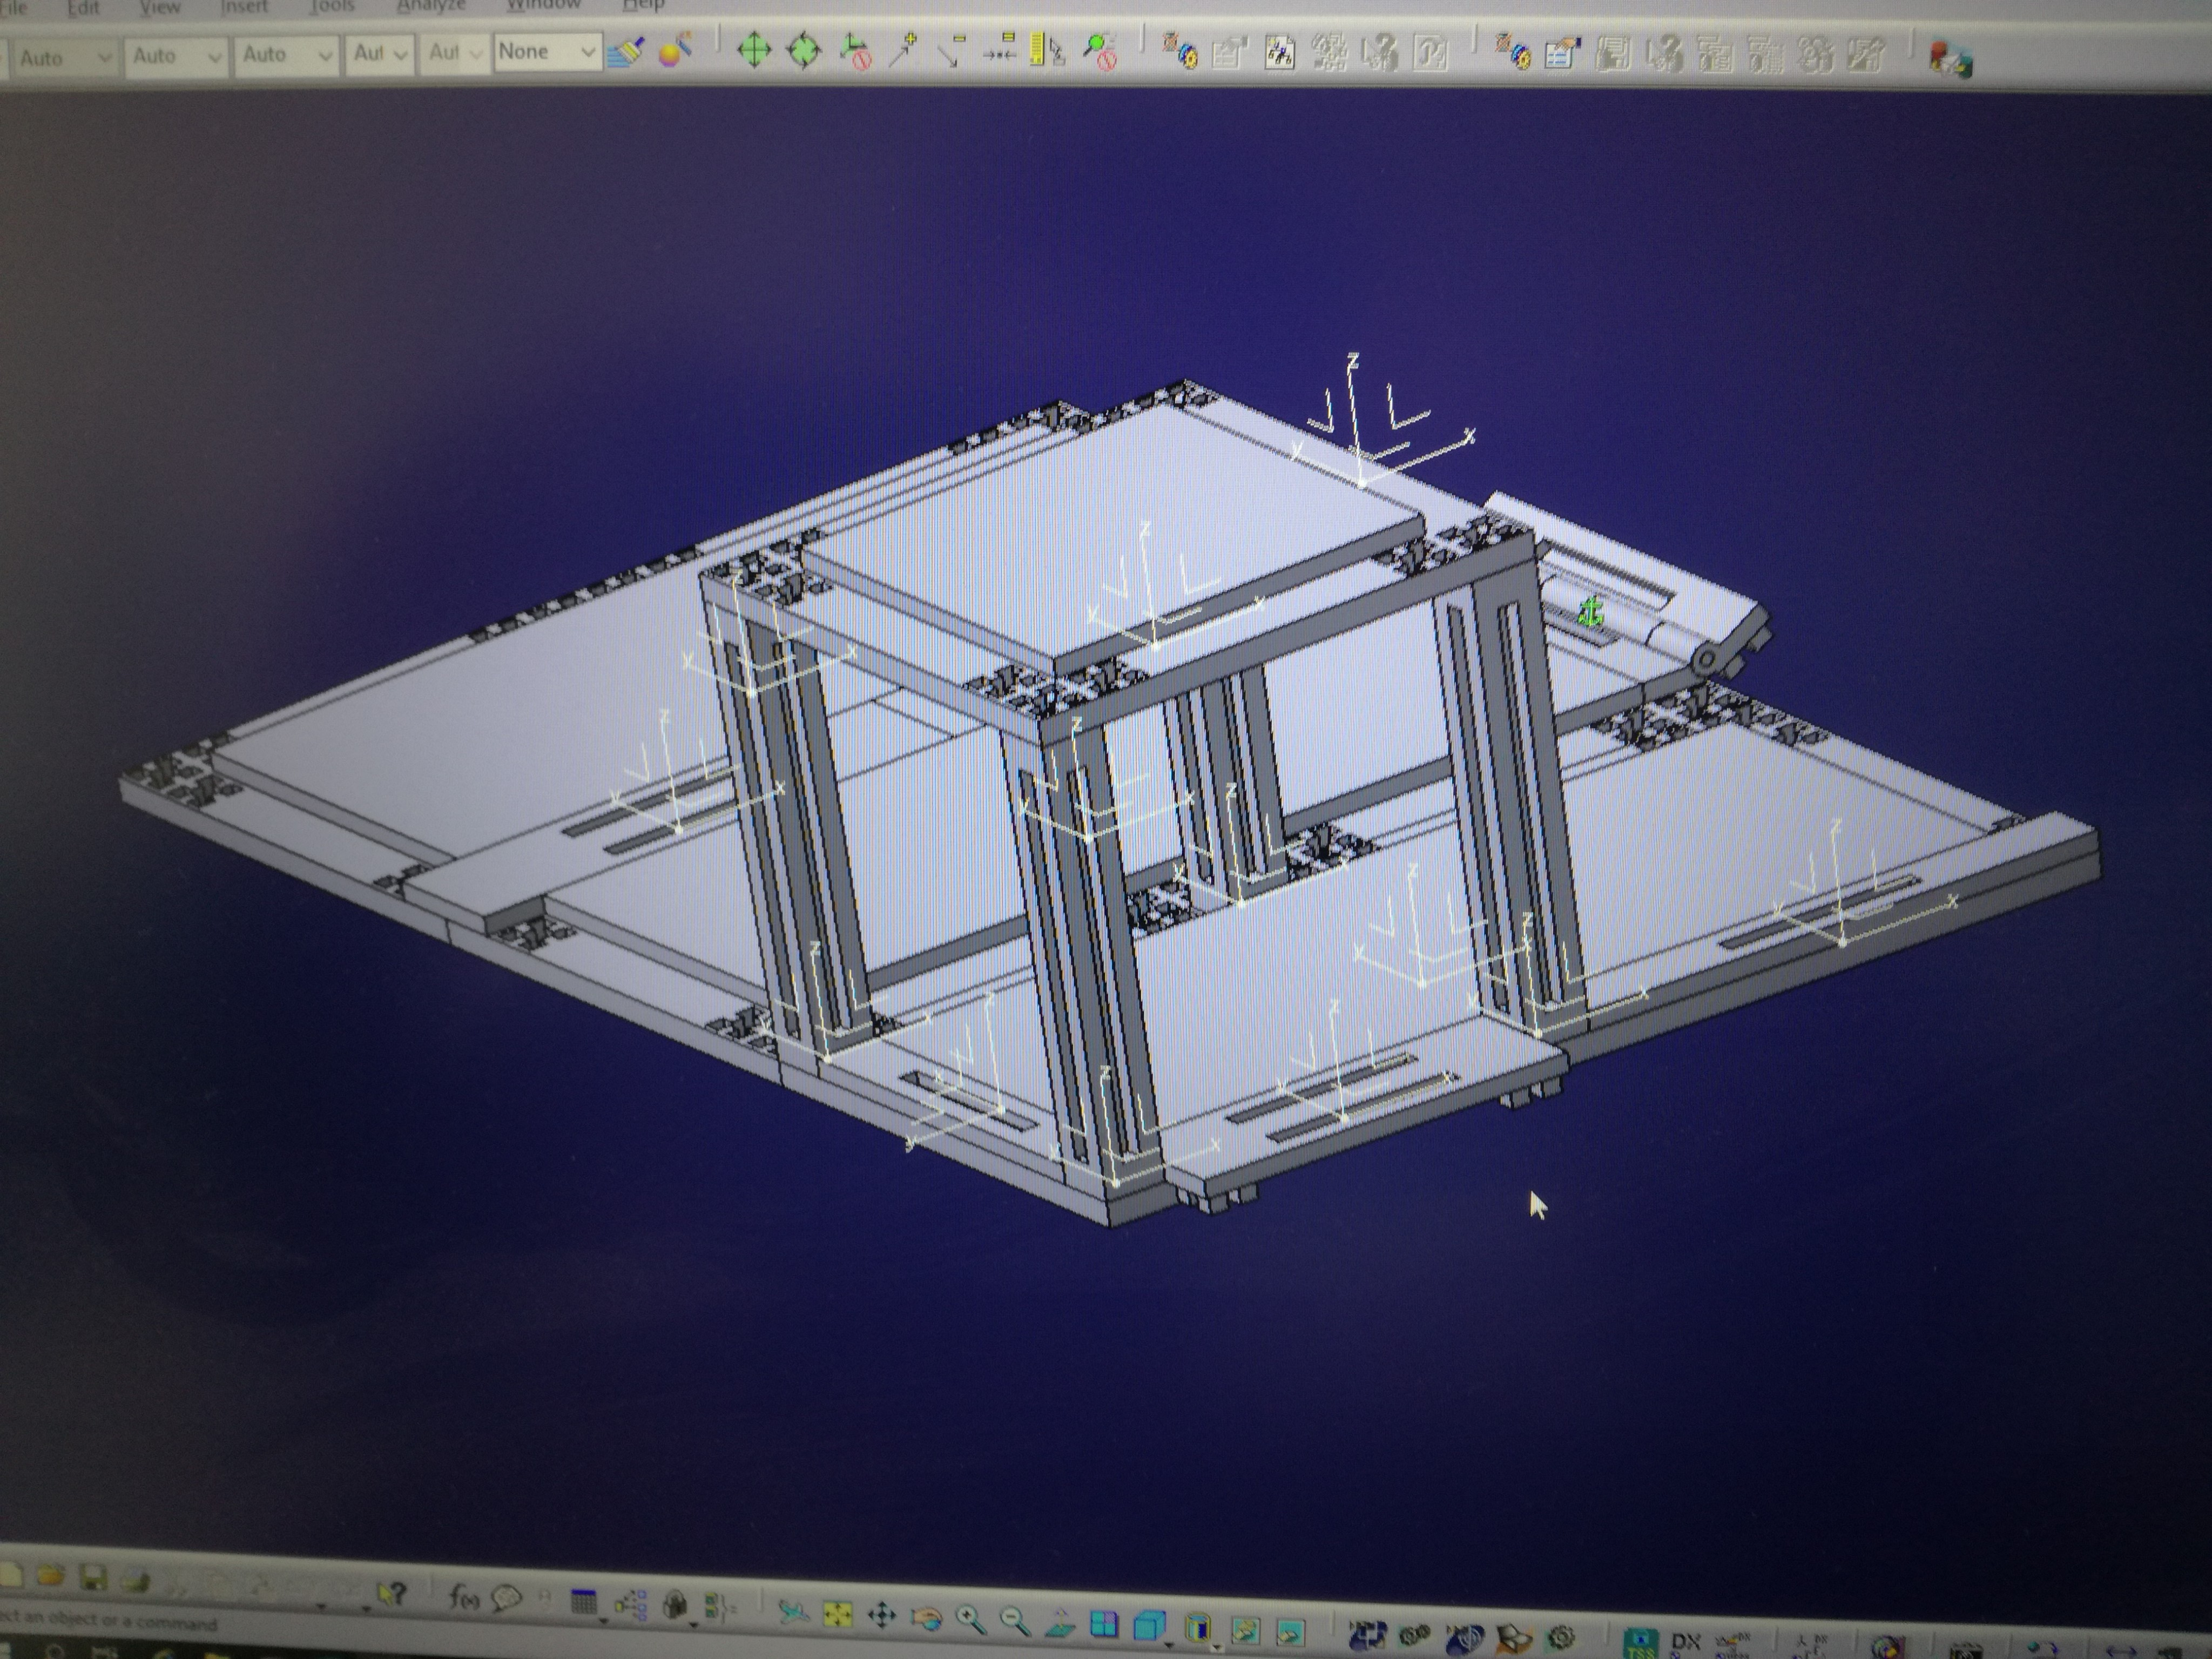
\includegraphics[width=0.45\textwidth]{fig_kniffelbot_8}
\end{center}

\end{frame}
%-----------------------------------------------------------------------------------------------------------

%-----------------------------------------------------------------------------------------------------------
\begin{frame}{Kosten bis jetzt}

\begin{center}
    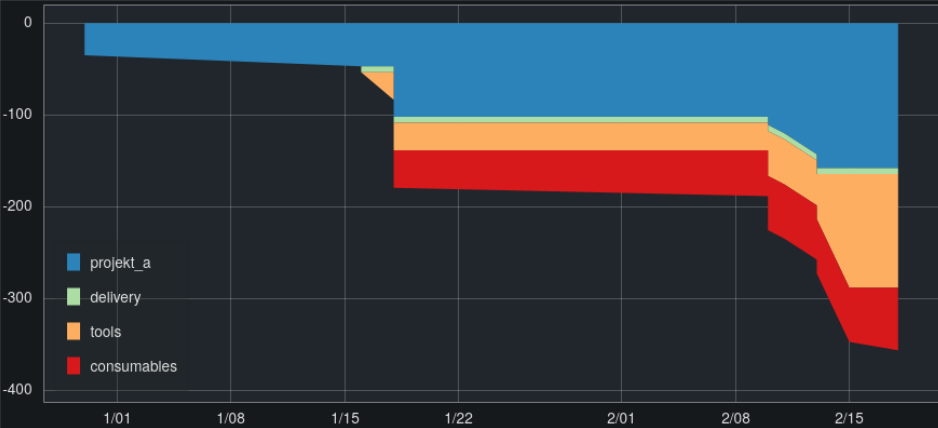
\includegraphics[width=\textwidth]{fig_kniffelbot_kosten}
\end{center}

\end{frame}
%-----------------------------------------------------------------------------------------------------------


%-----------------------------------------------------------------------------------------------------------
\begin{frame}{Kostendetails}

\begin{center}
    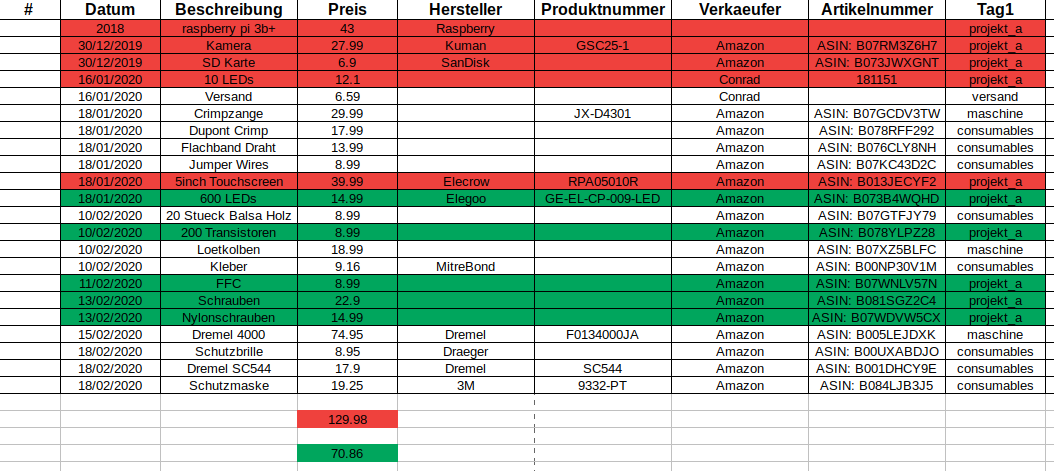
\includegraphics[width=\textwidth]{fig_kniffelbot_kosten_details}
\end{center}


\end{frame}
%-----------------------------------------------------------------------------------------------------------


%-----------------------------------------------------------------------------------------------------------
\begin{frame}{Wie gehts weiter?..}

\begin{exampleblock}{Supermodulares CAD:}
Ein modulares Korsett in welches alle Bauteile gesteckt werden: raspberry pi, camera, touchscreen. Stichwort: Lego f\"ur Erwachsene.\\
$\rightarrow$ Martin und Rob?
\end{exampleblock}

\begin{exampleblock}{3D Druck:}
Was ist technisch m\"oglich? Anfertigung!\\
$\rightarrow$ Simon im Austausch mit Martin und Rob?
\end{exampleblock}

\begin{exampleblock}{Hardware Version 2:}
Kann das billiger werden? Konkrete Vorschl\"age.\\
$\rightarrow$ Johannes im Austausch mit ... ?
\end{exampleblock}

\begin{exampleblock}{Software Version 2:}
Datenbank, Homepage, Methoden verbessern.\\
$\rightarrow$ Johannes im Austausch mit Daniel
\end{exampleblock}

\end{frame}
%-----------------------------------------------------------------------------------------------------------



%%%%%%%%%%%%%%%%%%%%%%%%%%%%%%%%%%%%%%%
\section{Quarant\"anegadgets}
%%%%%%%%%%%%%%%%%%%%%%%%%%%%%%%%%%%%%%%

%-----------------------------------------------------------------------------------------------------------
\begin{frame}{Projekte}

\begin{columns}[]

  \begin{column}{0.45\textwidth}
    
    \begin{alertblock}{projekt\_a:}
    Der Kniffelbot \phantom{p}
    \end{alertblock}
	
  \end{column}
  \begin{column}{0.45\textwidth}
    
    \begin{exampleblock}{projekt\_a2:}
    Weiteres einfaches Spiel?
    \end{exampleblock}
	
  \end{column}
\end{columns}

\begin{alertblock}{projekt\_b:}
Das Minigew\"achshaus: Frische Kr\"auter aus der eigenen K\"uche.\\
\begin{itemize}
 \item Was ist auf dem Markt?
 \item Wer sind die Kunden und was darf es kosten?
 \item Welche Technologie? Raspberry Pi vs Arduino?
 \item Prototyp?!
\end{itemize}
\end{alertblock}

\begin{columns}[]

  \begin{column}{0.45\textwidth}
    
    \begin{exampleblock}{projekt\_c:}
    Daniel hat ne prima Idee!
    \end{exampleblock}
	
  \end{column}
  \begin{column}{0.45\textwidth}
    
    \begin{exampleblock}{projekt\_d:}
    Johannes auch! \phantom{p}
    \end{exampleblock}
	
  \end{column}
\end{columns}

\end{frame}
%-----------------------------------------------------------------------------------------------------------


%%%%%%%%%%%%%%%%%%%%%%%%%%%%%%%%%%%%%%%
\section{Firmenstruktur}
%%%%%%%%%%%%%%%%%%%%%%%%%%%%%%%%%%%%%%%

\begin{frame}{Divide and Conquer}

\begin{alertblock}{Idee:}
Subgruppen unserer Gruppe k\"onnen verschiedene Sachen besser und schlechter. Teile in kleinere Teams f\"ur jeweilige Aufgaben, in welchen die Teilnehmer konkurrieren, aber dennoch immer wieder zusammenarbeiten und sich gegenseitig helfen.
\end{alertblock}

\end{frame}
%-----------------------------------------------------------------------------------------------------------

\begin{frame}{Aufgabenverteilung}

\begin{exampleblock}{Aufgaben:}
Ein Quarant\"anegadget besteht aus: Idee, Finanzplan, Hardware, Mechanik, Software, Elektronik, Marketing, Gesamtorganisation, Patente(?). 
\end{exampleblock}


\begin{alertblock}{Verteilung:}
\begin{columns}[]

  \begin{column}{0.45\textwidth}
 
    \begin{itemize}
    \item 00: Organisation
    \item 05: Ideen
    \item 10: Finanzplan
    \item 30: Elektronik
    \item 40: Mechanik
    \end{itemize}
	
  \end{column}
  \begin{column}{0.45\textwidth}
    
    \begin{itemize}
    \item 60: Prototypen
    \item 70: Patente
    \item 80: Homepage
    \item 90: Marketing
    \item 50: Software
    \end{itemize}
	
  \end{column}
\end{columns}
\end{alertblock}


\end{frame}
%-----------------------------------------------------------------------------------------------------------


\begin{frame}{Wie gehts weiter?..}

\begin{alertblock}{Hausaufgabe}
Vorschl\"age f\"ur
\begin{itemize}
 \item einen Namen
 \item ein Logo
\end{itemize}
\end{alertblock}

\begin{alertblock}{N\"achstes Treffen:}
Donnerstag, 09/04/2020 um 1730\\
Thema: Einteilen von Subgruppen und Aufteilen der Aufgaben
\end{alertblock}

\end{frame}
%-----------------------------------------------------------------------------------------------------------

\end{document}
%-----------------------------------------------------------------------------------------------------------
%---- END OF DOCUMENT ----------------------------------------------------------------------------
%-----------------------------------------------------------------------------------------------------------






